\section{Experiments with partitioned data and hierarchical models}
\label{sec:ep_application}

We apply the EP algorithm discussed in Section \ref{sec:ep_ep} to four different data sets, using a different hierarchical model for each data set. The first three data sets are simulated from known parameters while the fourth is an actual data set from astronomy, whose fitting involves developing a novel hierarchical mixture model with interpretable parameters. All MCMC runs, for either each of the EP sites or the full MCMC computation, use 4 chains with 1000 iterations, of which half are discarded as warmup.

% SIMULATED LINEAR REGRESSION
\subsection{Simulated hierarchical linear regression}
\label{subsec:ep_application_linear}

The first data set is simulated from a hierarchical linear model, our simplest example. Letting
$$ a_j = [\beta_{0j}, \beta_{1j}, \log \sigma_j]^T$$
denote the local parameters for each group $j$, we simulate $J = 50$ groups, with $I = 500$ data points per group, from
\begin{align}
a_{jp} &\sim N(\phi_p, e^{ \phi_{p+3} } ) && \\\nonumber
\epsilon_{ij} &\sim \normal(0,1) && \\\nonumber
y_{ij} &= \beta_{0j} + \beta_{1j} \cdot x_{ij} + \sigma_j \cdot \epsilon_{ij},
\end{align}
where $\beta_{0j}, \beta_{1j}$, and $\sigma_j$ correspond to the intercept, slope, and noise standard deviation for each group $j$; $\phi$ corresponds to the global parameter vector; and $x_{ij}$ are sampled from an arbitrary uniform distribution.

This problem has $3 \cdot 2 = 6$ shared parameters, $3 \cdot J = 150$ local parameters, and a total of $I \cdot J = 25,000$ samples. Our implementation uses R for the message passing framework and the Stan probabilistic modeling language \citep{Stan:2016} for MCMC sampling from the tilted distribution. We fit the hierarchical linear model with various EP settings, partitioning the data into $K = 5, 10, 25$ sites and running EP in both serial and parallel for each $K$. Uniform distributions are used as the initial site approximations, while a smoothing factor of $\delta=0.9$ is used in order to positive definiteness for each site approximation. We compare the results from the serial and distributed EP approximations to an MCMC approximation for the full model using Stan.

% SIMULATED SIGMOID
\subsection{Simulated hierarchical logistic regression}
\label{subsec:ep_application_logistic}

The next data set is simulated from a generalized inverse logistic (sigmoid) model. Letting
$$ a_j = [\beta_{0j}, \beta_{1j}, \log \sigma_j]^T$$
denote the local parameters for each group $j$, we simulate $J = 50$ groups, with $I = 500$ data points per group, from
\begin{align}
a_{jp} &\sim N(\phi_p, e^{ \phi_{p+5} } ) && \\\nonumber
\epsilon_{ij}  &\sim \normal(0,1) && \\\nonumber
y_{ij}  &= \beta_{0j} + \beta_{1j} \cdot \sigma \biggl( \frac{ x_{ij} - \mu_{1j} }{ \sigma_{1j} } \biggr) + \sigma_j \cdot \epsilon_{ij},
\end{align}
where $\sigma(\cdot) = \text{logit}^{-1}(\cdot)$; and $\beta_{1j}, \mu_{1j},$ and $\sigma_{1j}$ correspond to the maximal height, inflection point location, and (inverse) inflection point slope of the sigmoid in each group $j$.

This problem has $5 \cdot 2 = 10$ shared parameters, $5 \cdot J = 250$ local parameters, and a total of $I \cdot J = 25,000$ samples. As before, we use R and Stan for our implementation; we partition the data into $K = 5, 10, 25$ sites; and we compare the results from the EP approximations to an MCMC approximation for the full model using Stan.

% SIMULATED SIGMOID WITH DIP
\subsection{Simulated hierarchical logistic regression with Gaussian dip}
\label{subsec:ep_application_logistic_dip}

To add additional nonlinearities, for our last simulated data set we take the hierarchical sigmoid in Section \ref{subsec:ep_application_logistic} and multiply it by an inverted Gaussian, creating a "dip" in the regression curve. Letting
$$ a_j = [\beta_{0j}, \beta_{1j}, \mu_{1j}, \log \sigma_{1j}, \sigma^{-1}(\beta_{2j}), \mu_{2j}, \log \sigma_{2j}, \log \sigma_j]^T$$
denote the local parameters for each group $j$, we simulate $J = 50$ groups, with $I = 500$ data points per group, from
\begin{align}
a_{jp} &\sim N(\phi_p, e^{ \phi_{p+8} } ) && \\\nonumber
\epsilon_{ij} &\sim \normal(0,1) && \\\nonumber
y_{ij} &= \beta_{0j} + \beta_{1j} \sigma \biggl( \frac{ \log x_{ij} - \mu_{1j} }{ \sigma_{1j} } \biggr) \cdot \biggl( 1 - \beta_{2j} \exp \biggl( -\frac{1}{2} \bigg( \frac{ \log x_{ij} - \mu_{2j} }{ \sigma_{2j} } \biggr)^2 \biggr) \biggr) + \sigma_j \cdot \epsilon_{ij},
\end{align}
where $\mu_{2j}$ and $\sigma_{2j}$ correspond to the center and scale of the inverted Gaussian, while $\beta_{2j} \in [0,1]$ corresponds to the proportion by which the curve dips at the center of the Gaussian.

This problem has $8 \cdot 2 = 16$ shared parameters, $8 \cdot J = 400$ local parameters, and a total of $I \cdot J = 25,000$ samples. As before, we use R and Stan for our implementation; we partition the data into $K = 5, 10, 25$ sites; and we compare the results from the EP approximations to an MCMC approximation for the full model using Stan.

% ASTRONOMY DATA
\subsection{Galactic ultraviolet data}
\label{subsec:ep_application_astro}

Lastly, we demonstrate the EP algorithm applied to an actual data set in astronomy. The goal of our inference is to model the nonlinear relationship between diffuse Galactic far ultraviolet radiation (FUV) and 100-$\mu$m infrared emission (i100) in various regions of the observable universe. Data is collected from the Galaxy Evolution Explorer telescope. It has been shown that there is a linear relationship between FUV and i100 below i100 values of 8 MJy sr$^{-1}$ \citep{Hamden+others:2013}.  Here we attempt to model this relationship across the entire range of i100 values.

\begin{figure}
\centering
   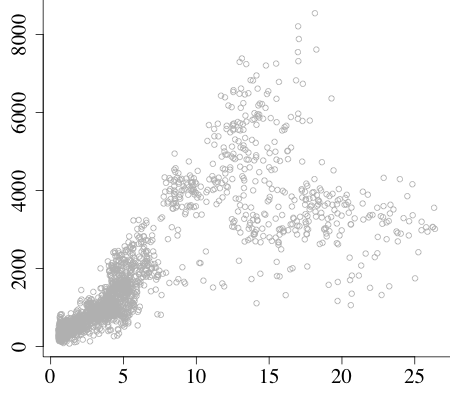
\includegraphics[width=0.33\textwidth]{figures/astro_data/1}
   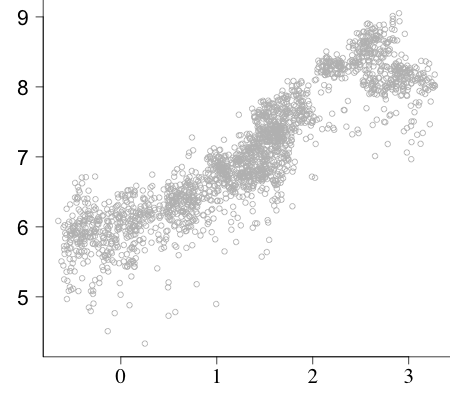
\includegraphics[width=0.33\textwidth]{figures/astro_data/1_log}
   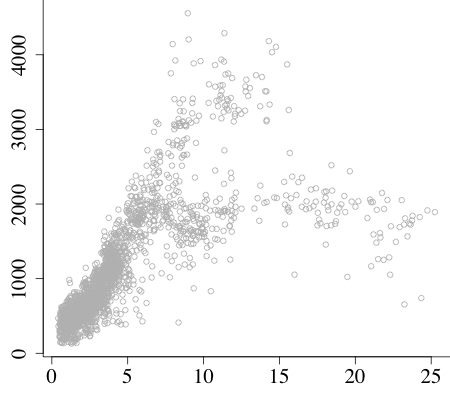
\includegraphics[width=0.33\textwidth]{figures/astro_data/2}
   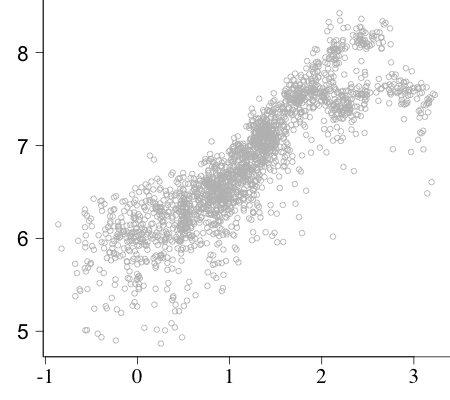
\includegraphics[width=0.33\textwidth]{figures/astro_data/2_log}
   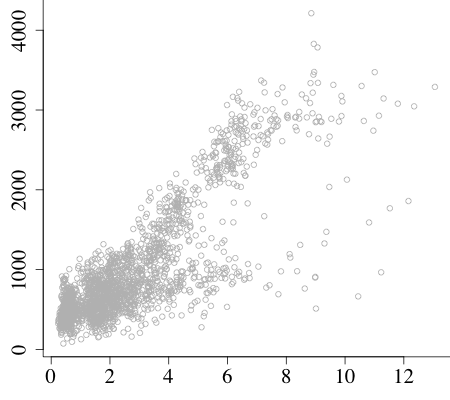
\includegraphics[width=0.33\textwidth]{figures/astro_data/3}
   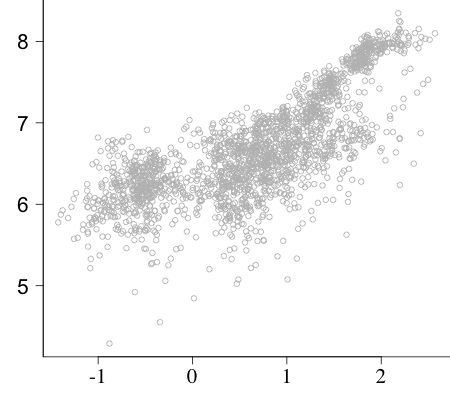
\includegraphics[width=0.33\textwidth]{figures/astro_data/3_log}
   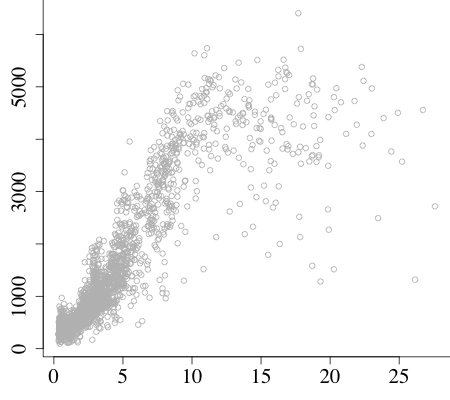
\includegraphics[width=0.33\textwidth]{figures/astro_data/4}
   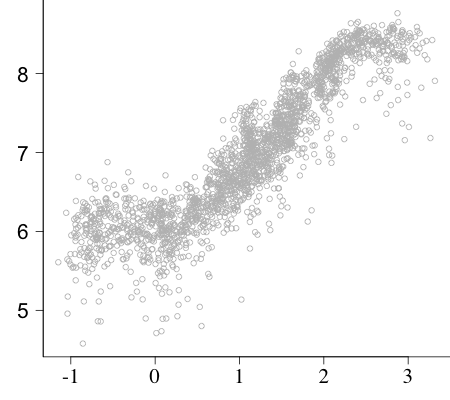
\includegraphics[width=0.33\textwidth]{figures/astro_data/4_log}
\caption{Scatterplots of ultraviolet radiation (FUV) versus infrared radiation (i100) in various regions of the universe. Data are shown for regions of longitude $12\degree, 23\degree, 92\degree$, and $337\degree$, and are presented with axes on the original scale (first column) and on the log scale (second column).}\label{fig:astro_data}
\end{figure}

Figure~\ref{fig:astro_data} shows scatterplots of FUV versus i100 in different longitudinal regions (each of width 1 degree) of the observable universe. The bifurcation in the scatterplots for i100 values greater than 8 MJy sr$^{-1}$ suggests a non-linear mixture model is necessary to capture the relationship between the two variables. At the same time, a flexible parametric model is desired to handle the various mixture shapes, while maintaining interpretability in the parameters.

Letting
$$ a_j = [\beta_{0j}, \beta_{1j}, \mu_{1j}, \log \sigma_{1j}, \sigma^{-1}(\beta_{2j}), \mu_{2j}, \log \sigma_{2j}, \sigma^{-1}(\pi_j), \log \sigma_j]^T$$
denote the local parameters for each group $j$, we model the top half of the bifurcation (i.e. the first component of the mixture) as a generalized inverse logistic function (as in Section \ref{subsec:ep_application_logistic}),
$$ f(a_j, x_{ij}) = \beta_{0j} + \beta_{1j} \sigma \biggl( \frac{ \log x_{ij} - \mu_{1j} }{ \sigma_{1j} } \biggr), $$
while the second mixture component is modeled as the same inverse logistic function multiplied by an inverted Gaussian (as in Section \ref{subsec:ep_application_logistic_dip}),
$$ g(a_j, x_{ij}) = \beta_{0j} + \beta_{1j} \sigma \biggl( \frac{ \log x_{ij} - \mu_{1j} }{ \sigma_{1j} } \biggr) \cdot
\biggl( 1 - \beta_{2j} \exp \biggl( -\frac{1}{2} \bigg( \frac{ \log x_{ij} - \mu_{2j} }{ \sigma_{2j} } \biggr)^2 \biggr) \biggr). $$
As such, the ultraviolet radiation ($y_{ij}$) is modeled as a function of infrared radiation ($x_{ij}$) through the following mixture model:
\begin{align}
    a_{jp} &\sim N(\phi_p, e^{ \phi_{p+9} } ) && \\\nonumber
    \epsilon_{ij} &\sim N(0,1) && \\\nonumber
    \log y_{ij} &= \pi_j \cdot f(a_j, x_{ij}) + (1 - \pi_j) \cdot g(a_j, x_{ij}) + \sigma_j \epsilon_{ij}, 
\end{align}
where $\pi_j \in [0,1]$ corresponds to the proportion of data generated by the first mixture.

This problem has $9 \cdot 2 = 18$ shared parameters of interest. The number of local parameters, however, depends on how finely we split the data in the observable universe. Our study in particular is constructed with $J = 360$ hierarchical groups (one for each longitudinal degree of width one degree), resulting in a total of $9 \cdot J = 3,240$ local parameters. We also sample the number of observations per group as $I = 2,000$, resulting in a total of $I \cdot J = 720,000$ samples. As for the simulated data, we use R and Stan for our implementation, and we compare the results from the EP approximations to an MCMC approximation for the full model using Stan. However, we partition the data into $K = 5, 10, 30$ sites because these values divide the $J = 360$ groups cleanly.
